% !TEX root = Projektdokumentation.tex
\section{Anhang}
\label{sec:Anhang}
\subsection{Gantt}
\label{app:Gantt}
\includegraphicsKeepAspectRatio{Bilder/Gantt.pdf}{1}
\clearpage

\subsection{Detaillierte Zeitplanung}
\label{app:Zeitplanung}
\tabelleAnhang{ZeitplanungKomplett}
\clearpage

\subsection{Use Case-Diagramm}
\label{app:UseCase}
\begin{figure}[htb]
\centering
% 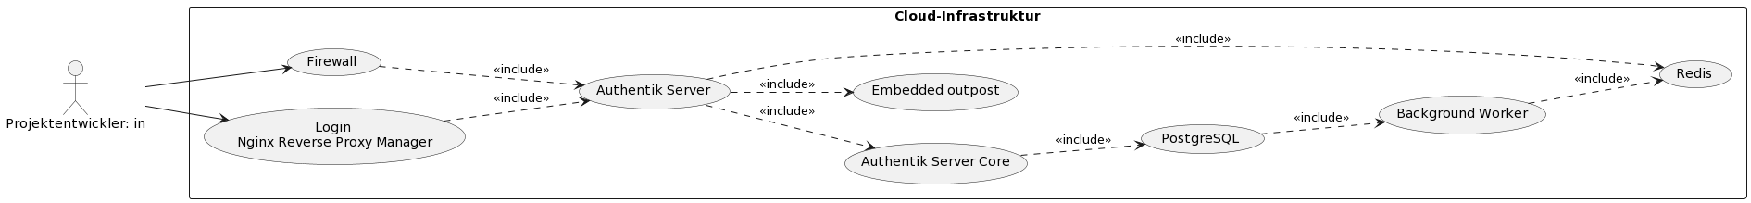
\includepdf[pages=-]{Use-Case-Diagram.pdf}
\rotatebox[origin=c]{90}{\includegraphicsKeepAspectRatio{Bilder/Use-Case-Diagram.pdf}{1}}
\caption{Use Case-Diagramm}
\end{figure}
\clearpage

\subsection{Sequenzdiagramm}
\label{app:Sequenzdiagramm}
% \includegraphicsKeepAspectRatio{Sequenzdiagramm.pdf}{1}

\subsection{Cloud-Infrastruktur}
\label{app:Cloud-Infrastruktur}
\includegraphicsKeepAspectRatio{Bilder/Cloud-Infra-Topology.png}{1}

\subsection{docker-compose.yml}
\label{app:docker-compose.yml}
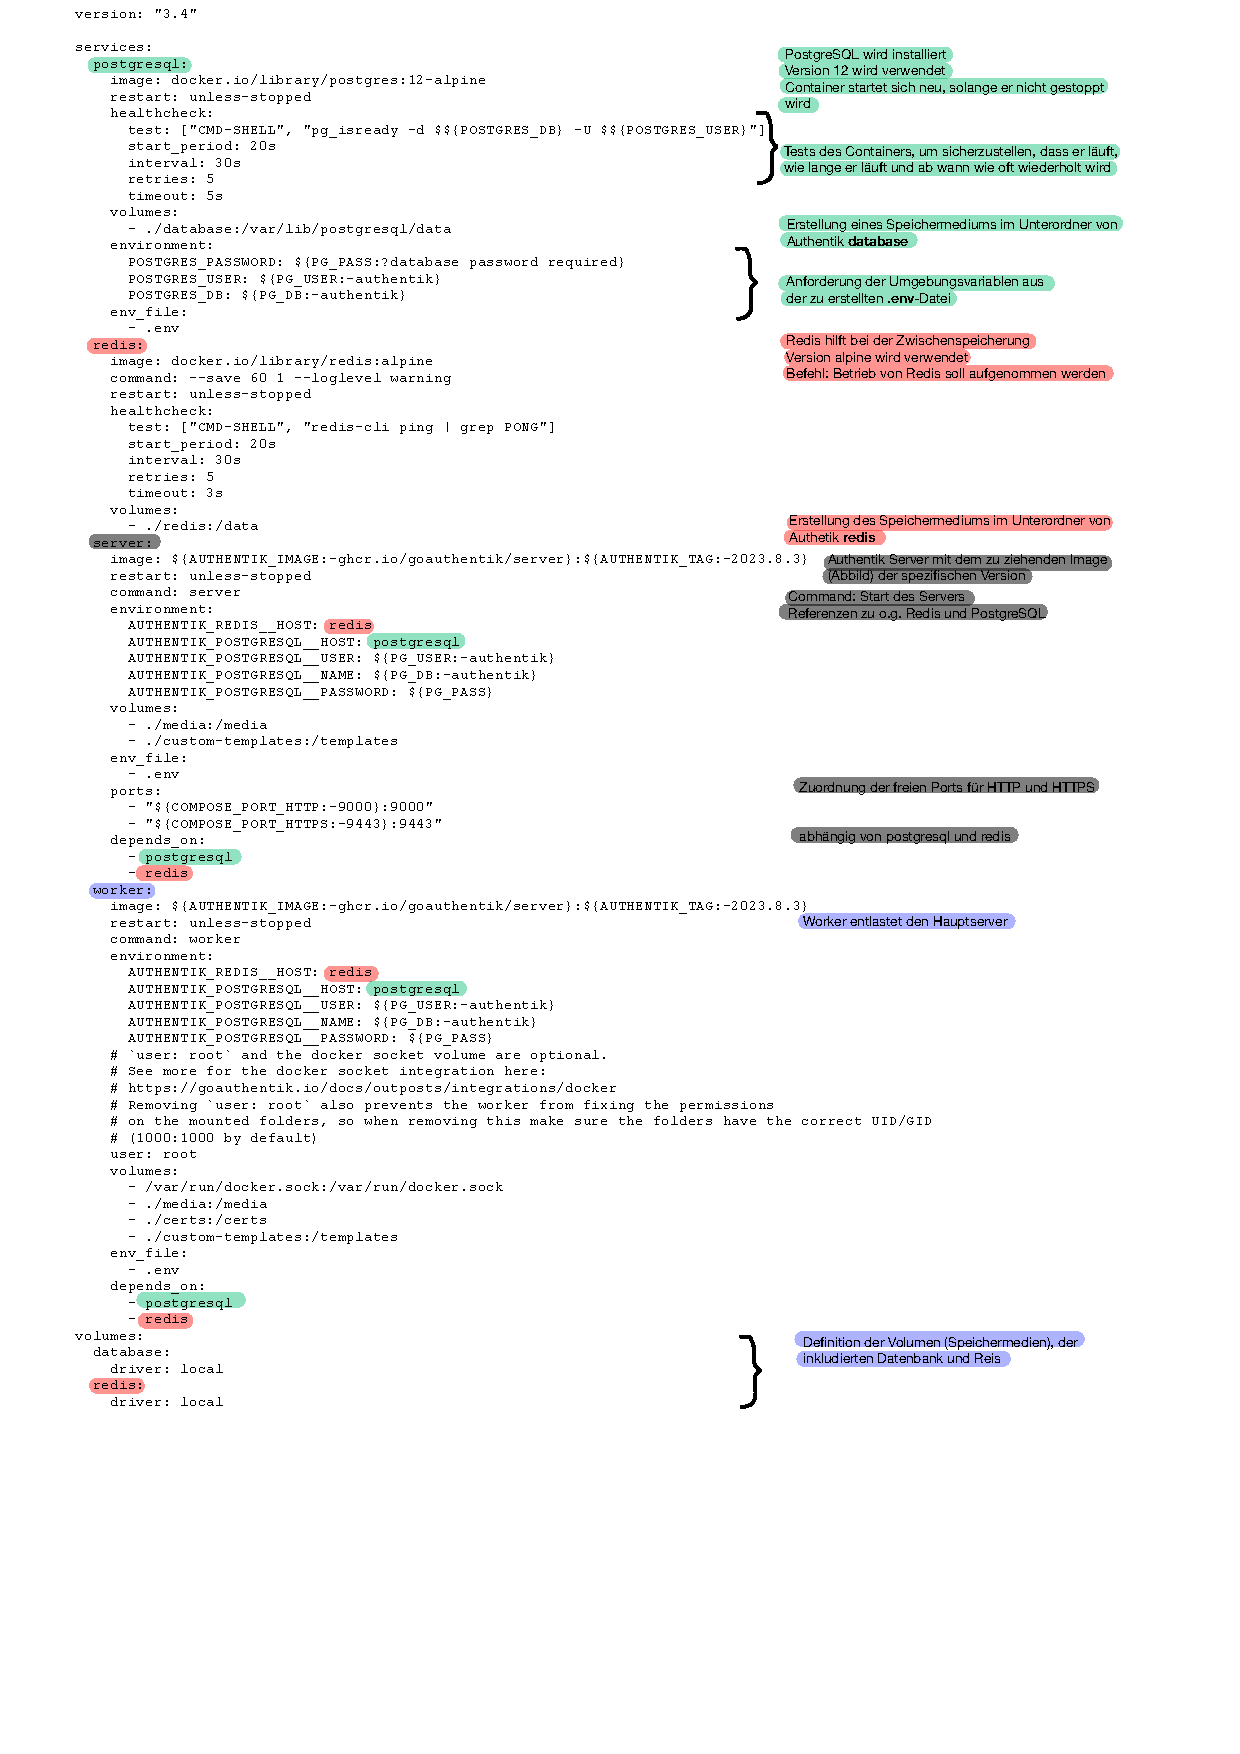
\includegraphics{Anhang/docker-compose.pdf}

\subsection{.env}
\label{app:dotenv}
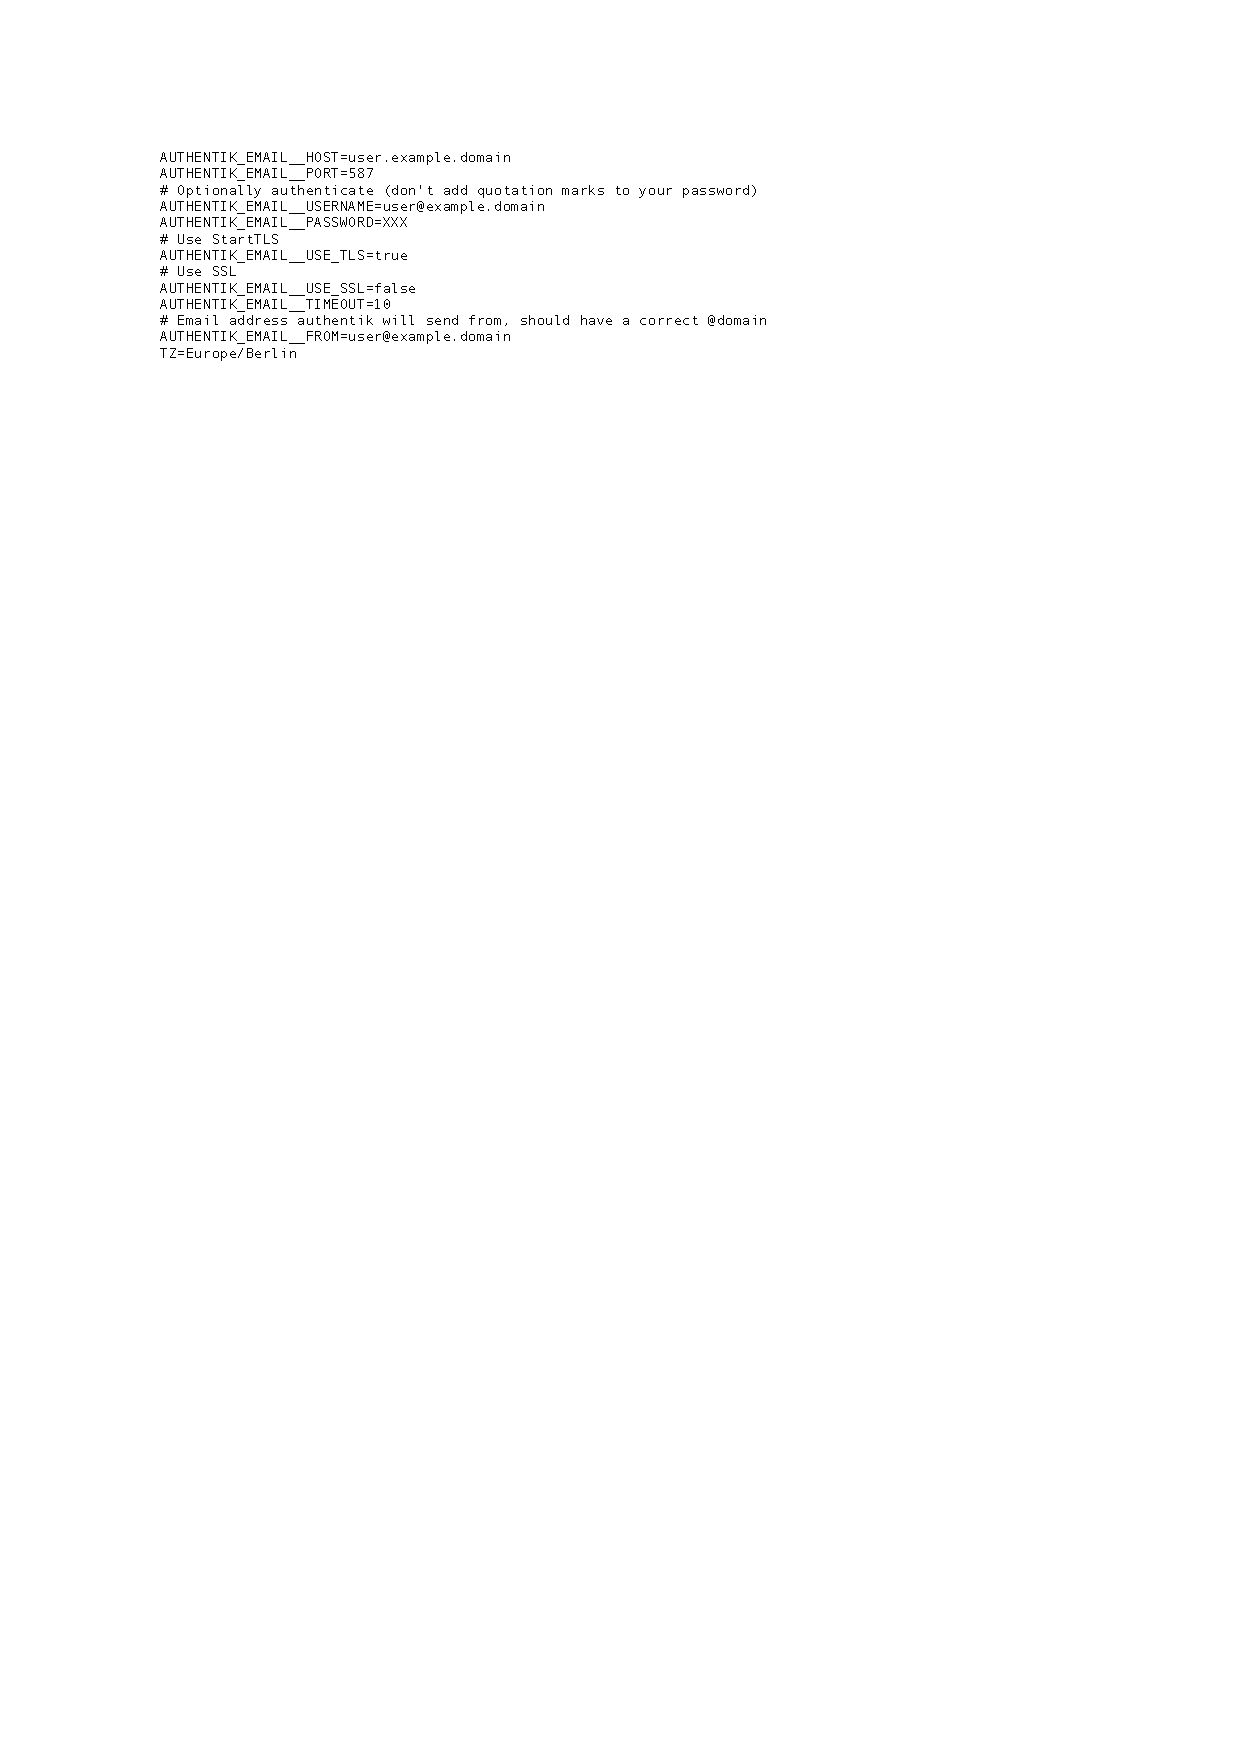
\includegraphics{Anhang/(.)env.pdf}

\subsection{NGinx Konfiguration}
\label{app:CustomNGinxConfig}
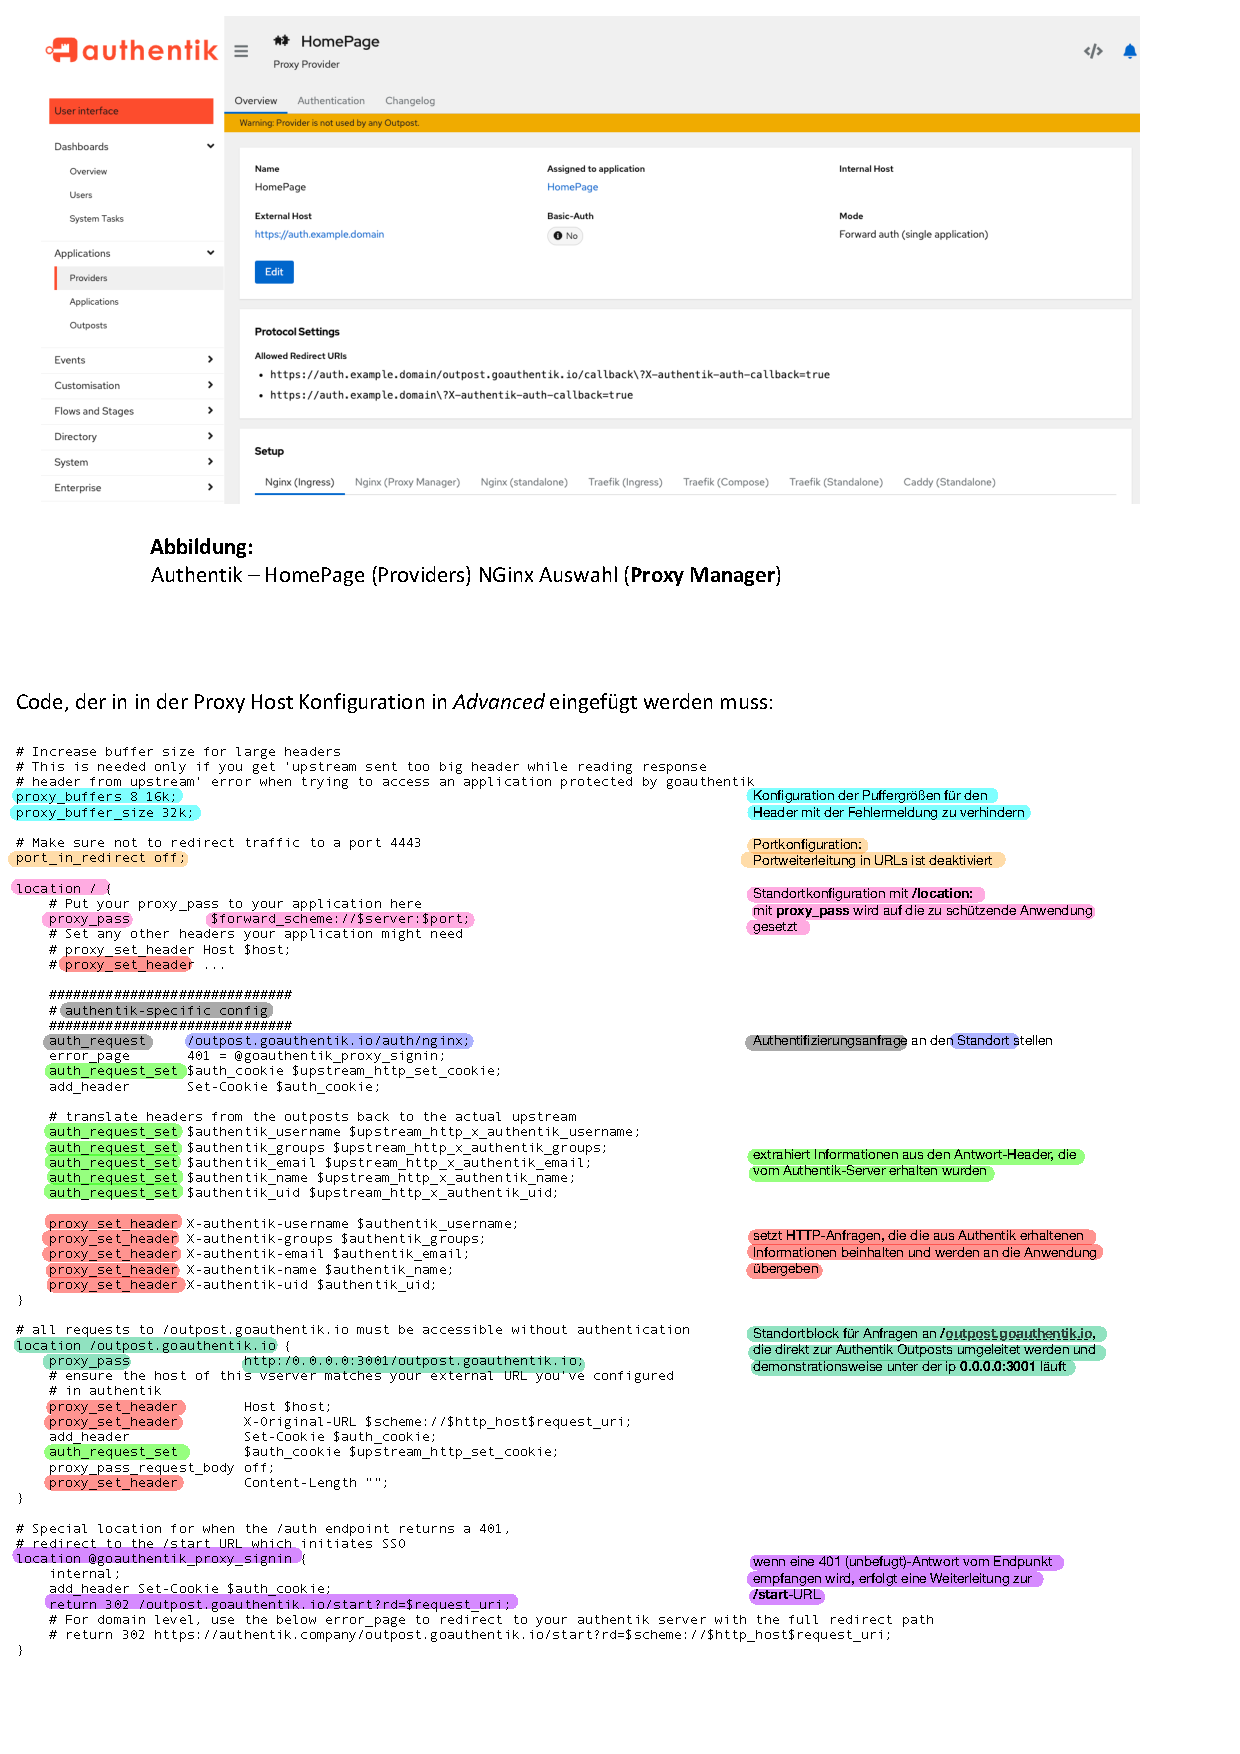
\includegraphics{Anhang/Custom_NGinx_Configuration.pdf}

\subsection{Benutzerdokumentation}
\label{app:Benutzerdokumentation}
\clearpage